\chapter{Installation on Linux and MAC OS X platform}\label{sec:InstallUnix}

\paragraph{}The FA$\mu$ST project is based on C++ library available for both UNIX and Windows environments. The proposed toolbox provides a Matlab wrapper. CMake has been chosen to build the project FA$\mu$ST because it is an open-source, cross-platform family of tools designed to build, test and package software. This chapter presents the steps to install the FA$\mu$ST tools on Unix platform (both Linux and Mac OS). 

\paragraph{}Please ensure that the \textbf{prerequisites components} listed in Section \ref{sec:RequiredTools} are installed. Then refer to the appropriate section : 
\begin{itemize}
\item Basic installation using \textbf{the command line terminal}, refer to Section \ref{sec:UnixBuildInstall}.
\item Basic installation using \textbf{the IDE "Code::Blocks"} for both Linux and MAC OS X, refer to Section \ref{sec:UnixInstallCodeBlock}. 
\item Basic installation using \textbf{the IDE "Xcode"} only on MAC OS X, refer to Section \ref{sec:MacInstallXcode}. 
\end{itemize}

Finally in Section \ref{sec:UnixCustomInstall}, the configure options available to build the FA$\mu$ST toolbox are described to propose an Custom - Advanced installation. For example, optional configuration can be activate such as modifying the install directory, or building in debug mode).  

\section{Required components}\label{sec:RequiredTools}
This Section lists the components required for FA$\mu$ST installation. 
\begin{itemize}
\item \textbf{Install CMake}. Visit the website \url{https://cmake.org/} to process to the installation.
\item \textbf{Verify Cmake install} by typing in a command terminal : 
\begin{lstlisting}
which cmake
\end{lstlisting}
The command terminal returns the path of your Cmake binary file like :
\begin{lstlisting}
/usr/bin/cmake
\end{lstlisting}
If not, add Cmake binary directory in the environment path. (in your ~/.bashrc file)

\item \textbf{Install Matlab} (\url{https://fr.mathworks.com/downloads/})

\item \textbf{Verify Matlab install} by typing in a terminal the following command : 
\begin{lstlisting}
which matlab
which mex
\end{lstlisting}
You must obtain the path of your matlab and mex binaries files like: 
\begin{lstlisting}
/usr/local/bin/matlab
/usr/local/bin/mex
\end{lstlisting}
If not, add \texttt{matlab} and \texttt{mex} binaries directories in your environment path (in your ~/.bashrc file). 

\item \textbf{export CC and CXX variables} corresponding to gcc and g++ binaries path :\\
find your gcc and g++ path using \texttt{which} command in a terminal :
\begin{lstlisting}
which gcc
which g++
\end{lstlisting}

Open your ~/.bashrc file and save the return-path of gcc and g++ like : \\
\begin{lstlisting}
# export version of gcc
export CC=/usr/lib64/ccache/gcc
export CXX=/usr/lib64/ccache/g++
\end{lstlisting}
\end{itemize}


\section{Basic build and installation}\label{sec:UnixBuildInstall}
\paragraph{}When prerequisities listed in precedent section \ref{sec:RequiredTools} are checked, the FA$\mu$ST installation can be done : 
if you are administrator of your machine (root access), follow instructions given in section \ref{sec:UnixBuildInstallAdmin}. Otherwise, for an local installation, refers to the section \ref{sec:UnixBuildInstallNOAdmin}. 

\subsection{Install with administrator privilege}\label{sec:UnixBuildInstallAdmin}

\begin{itemize}
\item \textbf{Download} the FA$\mu$ST package on the website :  \url{http://faust.gforge.inria.fr/}
\item \textbf{Open} a command terminal
\item \textbf{Set the current directory} to your FA$\mu$ST directory (NOTE: do not use any special character in your FAUST directory path, for example the character $\mu$)
\item Type the following commands : 
\begin{lstlisting}
mkdir build
cd build
cmake ..
make
sudo make install % run with administrator privilege
\end{lstlisting}
\end{itemize}

\paragraph{INFO:}When using the \textbf{cmake} command to generate the build system, \textbf{cmake} performs a list of tests to determine the system configuration and manage the build system. If the configuration is correct then the build system is generated and written. In this case, the three last lines of the console log of \textbf{cmake} command should be:
\begin{lstlisting}
-- Configuring done 
-- Generating done 
-- Build files have been written to: <YOUR/LOCAL/DIRECTORY/build>
\end{lstlisting}

\paragraph{INFO:}The command \textbf{make} will compile the build files.

\paragraph{INFO:}The command \textbf{sudo make install} will install the library and others components in the default directory: \\
\texttt{/usr/local/lib/libfaust.a} for the faust library, \\
\texttt{\textasciitilde /Documents/MATLAB/faust/} for the wrapper matlab.
\\
You must have administrator privilege because the library file \texttt{libfaust.a} is copied in an root path directory. If you do not have administrator privilege, you can make a local install (see. section \ref{sec:UnixBuildInstallNOAdmin}).

\subsection{Install without administrator privilege}\label{sec:UnixBuildInstallNOAdmin}

\begin{itemize}
\item \textbf{Download} the FA$\mu$ST package on the website :  \url{http://faust.gforge.inria.fr/}
\item \textbf{Open} a command terminal
\item \textbf{Set the current directory} to your FA$\mu$ST directory (NOTE: do not use any special character in your FAUST directory path, for example the character $\mu$)
\item Type the following commands : 
\begin{lstlisting}
mkdir build
cd build
cmake .. -DCMAKE_INSTALL_PREFIX="<Your/Install/Dir>"
make
make install
\end{lstlisting}
\end{itemize}

\paragraph{INFO:}When using the \textbf{cmake} command to generate the build system, \textbf{cmake} performs a list of tests to determine the system configuration and manage the build system. If the configuration is correct then the build system is generated and written. In this case, the three last lines of the console log of \textbf{•}{cmake} command should be: \begin{lstlisting}
-- Configuring done 
-- Generating done
-- Build files have been written to: <YOUR/LOCAL/DIRECTORY/build>
\end{lstlisting}

\paragraph{INFO:}The command \textbf{make} will compile the build files.

\paragraph{INFO:}The command \textbf{make install} will install the library and others components in the defined install directory. 






% CODEBLOCKS
\section{Build \& Install using Code Block}\label{sec:UnixInstallCodeBlock}
\paragraph{}When prerequisities listed in precedent section \ref{sec:RequiredTools} are checked, the FA$\mu$ST installation can be done : 

\begin{itemize}
\item \textbf{Download} the FA$\mu$ST package on the website :  \url{http://faust.gforge.inria.fr/}
\item \textbf{Open} a command terminal
\item \textbf{Set the current directory} to your FA$\mu$ST directory (NOTE: do not use any special character in your FAUST directory path, for example the character $\mu$)
\item Type the following commands : 
\begin{lstlisting}
mkdir build
cd build
cmake .. -G "CodeBlocks - Unix Makefiles" -DCMAKE_INSTALL_PREFIX="<Your/Install/Dir>"
\end{lstlisting}

\item Open the FAUST project from the file \textbf{./build/FAUST.cbp} with Code::Blocks IDE. 
\item In Code::Blocks IDE, select \textbf{ALL} target and build the project. 
\item In Code::Blocks IDE, select \textbf{install} target and build the project. 
\end{itemize}

\paragraph{INFO:}When using the \textbf{cmake} command to generate the build system, \texttt{cmake} performs a list of tests to determine the system configuration and manage the build system. If the configuration is correct then the build system is generated and written. In this case, the three last lines of the console log of \texttt{cmake} command should be:
\begin{lstlisting}
-- Configuring done 
-- Generating done 
-- Build files have been written to: <YOUR/LOCAL/DIRECTORY/build>
\end{lstlisting}
The optional parameter \texttt{$-G "CodeBlocks - Unix Makefiles"$} allows to generate the Code Blocks project and the Unix Makefiles. The optional parameter -DCMAKE\_INSTALL\_PREFIX="<Your/Install/Dir>" allows to install the binaries on the selected directory. If not used, the \texttt{make install} process must be realized with administrator privilege because the library file \texttt{libfaust.a} is copied in an root path directory. 


\section{Build \& Install using Xcode (for MAC OS)}\label{sec:MacInstallXcode}

The building with IDE Xcode concerns only MAC OS X environment.
\paragraph{}When prerequisities listed in precedent section \ref{sec:RequiredTools} are checked, the FA$\mu$ST installation can be done : 
\begin{itemize}
\item \textbf{Download} the FA$\mu$ST package on the website :  \url{http://faust.gforge.inria.fr/}
\item \textbf{Open} a command terminal
\item \textbf{Set the current directory} to your FA$\mu$ST directory (NOTE: do not use any special character in your FAUST directory path, for example the character $\mu$)
\item Type the following commands : 
\begin{lstlisting}
mkdir build
cd build
cmake .. -G "Xcode" -DCMAKE_INSTALL_PREFIX="<Your/Install/Dir>"
\end{lstlisting}

\item Open the FAUST project from the file \textbf{./build/FAUST.xcodeproj} with Xcode IDE. 
\item In Xcode IDE, select \textbf{ALL} target and build the project. 
\item In Xcode IDE, select \textbf{install} target and build the project. 
\end{itemize}

\paragraph{INFO:}When using the \textbf{cmake} command to generate the build system, \texttt{cmake} performs a list of tests to determine the system configuration and manage the build system. If the configuration is correct then the build system is generated and written. In this case, the three last lines of the console log of \texttt{cmake} command should be:
\begin{lstlisting}
-- Configuring done 
-- Generating done 
-- Build files have been written to: <YOUR/LOCAL/DIRECTORY/build>
\end{lstlisting}
The optional parameter \texttt{$-G "Xcode"$} allows to generate the XCode project. The optional parameter -DCMAKE\_INSTALL\_PREFIX="<Your/Install/Dir>" allows to install the binaries on the selected directory. If not used, the \texttt{make install} process must be realized with administrator privilege because the library file \texttt{libfaust.a} is copied in an root path directory. 


\paragraph{NOTE:}You can generated the target using the terminal command \texttt{xcodebuild} :
\begin{lstlisting}
mkdir build
cd build
cmake .. -G "Xcode"
%% list all target of the project
xcodebuild -list -project FAUST.xcodeproj 
%% Build the targets
xcodebuild -configuration "Release" -target "ALL_BUILD" build 
%% performs the "make install"
xcodebuild -configuration "Release" -target "install" build 
\end{lstlisting}




\section{Custom - Advanced Installation}\label{sec:UnixCustomInstall}

\paragraph{}The project FA$\mu$ST can be configured with optional parameters, for example if you want to install FA$\mu$ST in a different folder or to enable the parallel computing using multithread capacities provided by the OS. This build system can be parametrized using the Cmake Graphical User Interface, or the Cmake command line tools. 

\paragraph{}The Cmake Graphical User Interface ccmake allows you to select option input. When using the \texttt{ccmake} command in your build directory, the Cmake GUI appears in the console (see fig. \ref{fig:ccmake}).

\begin{figure}[!h] %%[!htbp]
\centering
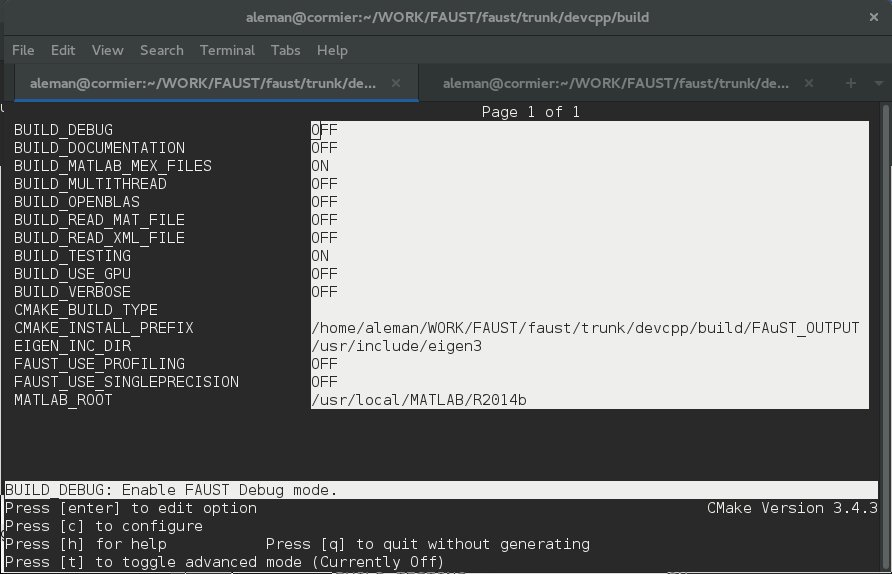
\includegraphics[scale=0.5]{images/ccmake.jpg}
\caption{ccmake GUI}
\label{fig:ccmake}
\end{figure}


%\section{Optional dependent tools}\label{sec:OptionalRequiredTools}
\paragraph{Optional Install of GPU process}
\begin{itemize}
\item \textbf{Install} CUDA and the drivers for NVIDIA.
\item \textbf{Verify install} of GPU tools by typing in a terminal : 
\begin{lstlisting}
which nvcc
\end{lstlisting}
You must obtain the path of your \texttt{nvcc} compiler like 
\begin{lstlisting}
/usr/local/cuda-7.5/bin/nvcc
\end{lstlisting}
If not, add \texttt{nvcc} directory in your environment path (in your ~/.bashrc file). 

\end{itemize}



\paragraph{}When scrolling on a value and pressing [enter], this value can be edited, the black underlaid row displays some information about the option and required path to create the build system. In the case of an option press [enter] to toggle the ON/OFF values. You can edit option by pressing [enter]. For example, press [enter] to edit option \texttt{CMAKE\_INSTALL\_PREFIX} to modify the install directory. 
\paragraph{}After choosing options for the build and setting the required fields, press [c] to configure. The configuration of the build system is checked again by Cmake, at the end of this check if the build settings are correct, you can press [g] in order to generate the build system.

\paragraph{} Instead the ccmake GUI, an other possibility to configure and generate the project is to use the command line cmake which can take the option input. Here is the list of available options: 
\texttt{$cmake\ ..\ -D<BUILD\_NAME>=<value>$}

\begin{itemize}
\item CMAKE\_INSTALL\_PREFIX : Install directory
\item CMAKE\_INSTALL\_MATLAB\_PREFIX : Install directory for the Matlab wrapper (mexfunction, demo ...)
\item BUILD\_TESTING : Enable the ctest option (default value is ON)
\item BUILD\_DOCUMENTATION : Generating the doxygen documentation (default value is OFF)  
\item BUILD\_MULTITHREAD : Enable multithread with OpenMP Multithreading (default value is OFF)
\item BUILD\_VERBOSE : Enable verbose option when compile (-v) (default value is OFF)
\item BUILD\_DEBUG : Enable FAUST Debug mode (default value is OFF )
\item BUILD\_USE\_GPU : Using both CPU and GPU process ( default value is OFF)
\item BUILD\_MATLAB\_MEX\_FILES : Enable building Matlab MEX files (default value is ON)
\item BUILD\_OPENBLAS : Using openBLAS for matrix and vector computations (default value is OFF )
\item BUILD\_READ\_XML\_FILE : Using xml2 library to read xml files (default value is OFF)
\item BUILD\_READ\_MAT\_FILE : Using matio library to read mat files (default value is OFF)
\end{itemize}

\paragraph{}Following the selected option, the cmake installer automatically checks the dependent component (library OpenBlas, eigen, matio, libxml2).  








\subsection{Required packages}\label{sec:RequiredPackages}

\paragraph{}Here is a list of packages used in the FA$\mu$ST project. The installation of this packages are automatically done. There are nothing to do. (see the directory "./externals").
\begin{itemize}
\item Library eigen \url{http://eigen.tuxfamily.org}
\item Library openBlas \url{http://www.openblas.net}
\item Library xml2 \url{http://xmlsoft.org}
\item Library matio \url{https://sourceforge.net/projects/matio}
\end{itemize}

\paragraph{Compatibility between MATLAB and compiler gcc} \textbf{Adjust your version of GCC compiler} in order to run the installation properly. The use of the mex function in Matlab requires that you have a third-party compiler installed on your system. The latest version of Matlab (2016a in our case) only supports up to GCC 4.7 (see \url{http://fr.mathworks.com/support/compilers/R2016a/index.html?sec=glnxa64} for more detail).
